%---------- Inleiding ---------------------------------------------------------

\section{Introduction}
\label{sec:introduction}

% Rope skipping is een evoluerende jurysport. Jaar na jaar neemt de concurrentie toe met moeilijkere en meer gevarieerde skills. 
% Door de toenemende populariteit van beeldherkenning, krachtigere CPU's en GPU's, en toepassingen die objecten in afbeeldingen herkennen \autocite{Singh_Gill_2022} 
% of acties in video's detecteren \autocite{LUQMAN_2022}, werd zich afgevraagd of dit ook van toepassing kan zijn op meer gecompliceerde en gevarieerd beeldmateriaal.
    
% Op rope skipping competities worden winnaars bekroond door een panel  juryleden die de freestyle van een springer beoordelen. Door groeiende concurrentie, meer gevarieerde trucs, snellere uitvoering en stijgende moeilijkheidsgraad, wordt het jureren lastiger. We onderzoeken of huidige \emph{computer vision}~\ref{subsec:computer vision} technieken klaar zijn om op basis van beeldmateriaal skills te herkennen en deze in te zetten om de objectiviteit en correctheid van scores te verhogen. Verder kan de trucherkenning gebruikt worden om de toeschouwer meer transparantie te bieden de puntentelling, door een replay af te spelen met skill- en scorebenoeming.
Jump rope is an evolving sport.
Year after year, an increasing amount of high-level competitors are pushing the limits of jump rope.
% TODO : source?
This results in new skills, new combinations, better physiques, better rope material, and faster movements. For the judges to keep up with the jumpers and to correctly assess scores to a routine, Double Dutch freestyles\footnote{Two turners, with one or more jumpers} are reviewed at half speed in International competitions or even at nationals in Belgium.

Head judges around the world question the best way to judge athletes correctly as to give an accurate and objective ranking on national or international competitions.
Many solutions have been provided: another judging rule-set\footnote{The current rule-set is enforced and maintained by \href{https://www.gymfed.be/}{Gymfed}, closely related to the international judging-rules from the \href{https://ijru.sport/}{International Jump Rope Federation}}, splitting judge responsibility, replaying the routine at half speed \dots
However, with the increasing popularity of image recognition, more powerful computers, applications that recognize objects in images \autocite{Singh_Gill_2022}, implementations detecting simple human actions \autocite{LUQMAN_2022} and the successful test of \href{https://nextjump.app/}{NextJump}s AI speed-counter, they wondered about the possibility of incorporating artificial intelligence into jump rope freestyles.

This raises some questions when trying to answer the main research question of this paper: \textbf{``How can artificial intelligence be incorporated into jump rope freestyles to increase the objectiveness and accuracy of judging?''}.

\subsection{Problem domain}

Jump rope, like gymnastics or athletics, exists in many disciplines, e.g. Speed, Single Rope freestyle (single/pair/team), Chinese Wheel (CW), Double Dutch (single/pair) \dots. To accurately judge routines, each discipline has its own rules. Although interlapped, differences exists. Each athlete or team then performs a choreography of 60 to 75 seconds showcasing their favorite skills and uniqueness.

\subsubsection{What are the challenges for judges today?}

On competitions, judges watch the routine live to annotate the difficulty or creativity. Each judge pays attention to his assigned part with the athletes, all contributing to the total score of the freestyle. to keep up, double dutch diff judges\footnote{Those judges judging the difficulty of double dutch routines.} are already allowed to review routines at half speed in order to accurately score them.

\subsubsection{How is difficulty scored?}

Performed skills al have a level, which will be written down when seen by the judge. Each level also has a numeric score contributing to te total difficulty of the routine. Judges see and calculate/memorize the level of each skill, write it down, count the amount of levels jumped and calculate the diff score.

\subsubsection{What can be done to increase the accuracy of judging?}

Increasing the judging accuracy and fairness can be done on multiple levels. Adding more judges, each specializing in their own field, finetuning or adapting the rules or reviewing at half speed are all things that can or are applied. % TODO : abrubt end?

\subsubsection{How can machine learning be integrated into jump rope freestyles}

% TODO : footnote nextjump, incorporate more results?
The preferred solution in this proposal is an AI-model recognizing (sub)skills and transitions in a double dutch single freestyle (DD3) as assigning correct levels at world championships or even nationals in Belgium is perceived to be hard and the current main issue.

\subsubsection{Which data is available for the AI to use?}

To recognize hundreds of skills, variations and transitions, lots of data is needed. Both individual and team freestyles are mostly recorded by clubs themselves or from the given organization, some which are available on social media. The task is to explore and gather as much as possible. 

\subsubsection{When are AI-recognitions acceptable to potentially use on competitions?}

Judges do make mistakes, just like the AI models, but we do need a baseline for an acceptable result. Competition scores can be used to define a target.

% TODO : mention speedcounter 10h - 36h speed accurate vs triples, double unders accurate in literature

\subsection{Solution domain}

Until now, only the scope has been narrowed. The literature, implementation \& labeling will give more clarification on different questions. Getting to know the topic is great, but this doesn't get us further into the solution. Let's jump into it.

\subsubsection{What are the skills and transitions that need to be recognized?}
% TODO : provide examples of skills
For double dutch, there are two turners and a jumper. All three of them act as a unit and execute skills such as a frog, push-up or a cartwheel. Turners can then increase the difficulty by turning in a cross, on the back or two ropes underneath the jumper at once. But even the jumper can make transitions like a turntable, which is the same skill but then your body position changes a quarter or even more. Further clarification in the literature review.

\subsubsection{What would be a minimal Proof of Concept (PoC)?}

The PoC would be a model recognizing the most common skills and transitions.
This means omitting or just marking special combinations, longer double dutch switches or long time sequences of emptiness in general. But the PoC should preferably be able to generalize uncommon skills that are still definable as normal. Better described would be knocking on the door three times, someones at the door, but knocking four times or with a bonk in between is also recognizable.

\subsubsection{Which human activity recognition examples can be used or altered as the base of the model/research to pick out the best ones?}
% TODO : source source source
Quick searches give you examples of object recognition, detecting sign language \dots
These implementations can be used as a first base.
Examples give the idea that data mostly seem more to be centered, which is not the case in jump rope videos, a solution need to be found for that. The second problem is that freestyles can consist of more than fifty different skills, which takes to long to cut manually.

\subsubsection{How much data is expected to increase the accuracy off the Judge?}

The amount of videos will keep rising, but will the current amount be sufficient? If its not enough, how much more would be expected and what about uncommon skills. Do we need to specially record them? But what about new skills on competitions?

\subsection{Additional questions}

The proof of concept will probably raise a lot of questions as a byproduct such as:

\begin{itemize}
    \item How can we use the AI-Judge to improve judges?
    \item What needs to change on a working model, to apply it on other judge-related sports such as gymnastics, synchronized swimming, figure skating \dots
\end{itemize}


\subsection{Introduction summary}

With basic knowledge about jump rope and the goal of paper, further research, (label)definitions, modelselection and implementation can be performed. Let's start by exploring earlier work while slowly increasing more jump rope definitions.



%---------- Stand van zaken ---------------------------------------------------

\section{Literature review}%
\label{sec:literature}

% TODO: (TAAL controle literatuur)

% TODO BP: volgorde en uitbreiding literatuur.
% Convolutielagen in een nutshell -> van matrix naar matrix (afbeelding), maar cellen van een nieuwe matrix zijn een som van andere rijen en kolommen (initieel pixels)
% LSTM in een nutshell -> geheugencellen, activatiefunctie -> input, memory, activativering output.
    
Het onderzoek naar skillherkenning wordt stapsgewijs opgebouwd. Beginnen doen we met een introductie en definitie van skills, waarna gepast onderzoek naar technieken kan gebeuren. Stilaan bouwen we dit op tot we beter definiëren waar de moeilijkheden liggen bij het herkennen van skills om zo de gevonden modellen te verfijnen tot het gewenste resultaat.

The research towards skillrecognition will be done in step by step. First is an introduction and definition of skills, secondly which challenges and how the data will be repre ... % TODO : further translate depening on the shuffled introduction and literature

\subsubsection{Speed record table}

\subsection{Skills intro}
\label{subsec:basisskills}

% Eerder beschreven we al de aanwezigheid van verschillende onderdelen in Rope Skipping. Om het onderzoek doenbaar te houden, leggen we de focus op single rope individuele freestyle (SR) en double dutch single freestyle (DD3). Beide onderdelen hebben een ander jurysysteem, waarbij verschillende elementen terugkeren, maar ook anders zijn. Soms wordt ook enkel over SR gesproken om niet in herhaling te vallen.

Earlier we described the presence of multiple disciplines in Jump Rope. To keep the research doable, freestyle skill recognition will be start on one discipline. The main candidates for freestyle skill labeling will be single rope and double dutch single freestyles. Bot judging systems incorporate their own rules, where overlap/similarity of skill movements are common. 

\subsubsection{Single Rope - SR}

Single Rope is the style defined where jumpers use their individual rope to execute different skills belonging divided in categories: gymnastics G, powers P, wraps W, releases R, backwards B, multiples M, crosses C, footwork F, Interactions I and an endless possibility of combinations. Multiples for example are actually multiple crosses in one jump. Likewise, releases can be combined with wraps, multiples with powers and so on.

Some examples:

% TODO : bijlage bij BP
\begin{itemize}
    \item Crosses
    \begin{itemize}
        \item side swing (s - swing next to the body)
        \item open (o - normal jump)
        \item cross (c - crossed arms on the stomach)
        \item toad (raise knee, other arm under your knee)
        \item EB (arm on stomach + arm on back)
        \item AS (arms crossed behind the knees)
        \item CL (one arm behind the knees, other on the back)
        \item TS (arms crossed behind the back)
    \end{itemize}
    \item Multiples
    \begin{itemize}
        \item double - DU - 2 rotations
        \item triple - TU - 3 rotations
        \item quad - QU - 4 rotations
        \item quint - 5 rotations
        \item TU.s.EB.o - first rotation on the side, next EB, next open
    \end{itemize}
    \item Powers
    \begin{itemize}
        \item push-up - to plank position and pushing upwards while pulling the rope underneath your feet.
        \item split - idem push-up, but to split
        \item frog - handstand
    \end{itemize}
\end{itemize}

Each skill will then be assigned a level contributing to a score. 

\subsubsection{Double Dutch - DD}
\label{subsubsec:double dutch}

Double Dutch consists of two turners and one jumper alternating rope rotations. Elements in Double Dutch are similar, but different at the same time. The jumper does all the skills, mainly powers, gymnastics or footwork, since he doesn't need to hold the rope. Turners can manipulate the rope using multiple unders, turnerskills like crossed arms, EB, toad\dots or even involve gymnastics themselves.
To judge double dutch, snapshots are taken, then the level will be given depending on the combination of turnerskills, jumperskills and roperotations.
Switching turners also contributes to scoring.

Like any discipline, mistakes can happen, they'll be deducted from the total score.

\subsection{Computer vision}
\label{subsec:computer vision}

% TODO : footnote refer to table above for numeric data
To recognize the skills automatically input data is needed. There are quite some videos on socials, as well as in-house recordings \ref{tbl:data-comparison}, so the choice to learn from videos was made quickly. The field of study in which computers recognize features, people or other objects in digital imagery is called computer vision. More specifically, the focus is recognizing human actions in these recordings, called human activitity recognition or HAR \autocite{Pareek_2020}.

Human Gait Recognition, HGR, or Human Pose Estimation, HPE, are also used to recognize human activities. Although the three techniques are closely related, each has a different nuance. Gait recognition looks at a person's typical movements, gestures or behavioral patterns \autocite{Alharthi_2019}, while pose estimation looks specifically at poses or special expressions \autocite{Song_2021}. They also talk about how pose recognition, skeleton-based, can be used as a tool are to improve activity labeling.

Models providing skeleton-structure or others can be used to improve action recognition, mainly because crosses, powers, releases\dots are build from these poses.

\subsection{HAR general progress}

% TODO : find paper, reference to come to steps or use pareek again?
The following approach is mainly formed after reading the survey of \textcite{Pareek_2020}, he describes the recent updates in human activity recognition.

\begin{enumerate}
    \item Jumper localization
    \item Action segmentation, start of skill, end of skill
    \item Predict level or variation element (multiple, cross, gym...)
    \item Predict the effective skill
\end{enumerate}

Jumpers can stand everywhere in the field, in order to perform better, locating and cutting out the athlete can improve the segmentation model. When the skippers are centered, better action segmentation can be performed. This allows predicting skills on newly recorded videos, without needing to cut out the different skills. Finally predicting the skill.

\subsection{Jumper localization}
\label{subsec:jumper localization}

% Het eerste doel van het proefconcept is het herkennen van de springer. \autocite{Zaidi_2021} deed een onderzoek naar de moderne deep learning technieken voor het herkennen van objecten en besprak verscheidene modellen, zoals YOLO, SSD, CenterNet, CNN, hun varianten en de nood aan compactere modellen voor dagelijks gebuik. Echter vergt het onderzoek niet het herkennnen van rope skippers op één afbeelding, maar gedurende de gehele video of videofragmenten. Om dit proces mogelijk te vereenvoudigen vergelijkt \textcite{Gao_2022} recente deep learning technieken die de voor- en achtergrond in video's van elkaar onderscheiden, genaamd video object segmentation of VOS. Gaande van het herkennen van een persoon, tot het herkennen van armen, benen, voeten, handvaten en touwen. Hoewel \textcite{Bharadiya_2023} aangeeft dat CNN kenmerken herkent ongeacht de positie in de afbeelding, zouden we de gemaskeerde beelden kunnen schalen en centreren. Vooral bij wedstrijddata springen atleten dichtbij of ver in het veld ten opzichte van de camera. In het volgende deel kunnen we dit dan gebruiken voor volledige trucherkenning.

Many research towards image recognition has been done \autocite{Zou_2023}. The best models mostly utilize Convolutional Neural Networks pertaining spacial information in the image \autocite{Zaidi_2021}. In their paper, they compare some recent models for object detection such as YOLO(v4), CenterNet, SSD, EfficientDet-D2, each using some backbone architecture like VGG-16, AlexNet, GoogleNet or lightweight models such as ShuffleNet or MobileNet (all using CNN's). Some of them being real-time models (fps > 30).
The goal of localizing the jumper is to center the athletes in the middle of the screen/video. \textcite{Bharadiya_2023} elaborates that the position of objects in images doesn't really matter, but their are no clear statements about the size of objects. It could be that a jumper takes up 80 percent of the screen, while moments later he moved backwards and only takes up 30 percent of the video. Instincts tell us that centered and scaled data will work better later.

One of these models can be taken as a base, using transfer learning\footnote{Concept transfer learning explained in \autocite{Bharadiya_2023}} to fine-tune the results to localize the jumper.

To improve localization, video object segmentation or video instance segmentation can be used. \textcite{Gao_2022} lists some object segmentation models, like SwitNet \textcite{Wang_2021} using ResNet18 as good and quick model.
Other possibilities would be Cutie \autocite{Cheng_2023}, DensePose (see fig [\ref{fig:srwrap}, \ref{fig:srwrapdense}]) \autocite{Guler_2018}

\begin{figure}
    \centering
    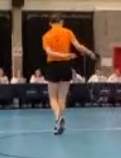
\includegraphics[width=0.3\linewidth]{img/sr_wrap}
    \caption{Jumper wrapping the rope, SR}
    \label{fig:srwrap}
\end{figure}

\begin{figure}
    \centering
    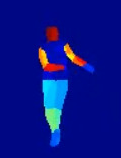
\includegraphics[width=0.3\linewidth]{img/sr_wrap_dense}
    \caption{Jumper wrapping the rope, denseposed}
    \label{fig:srwrapdense}
\end{figure}

Densepose seems to be able to give the bounding boxes of the main poses detected. Perhaps just a convex hull and some padding will be enough for smart cropping and training a network from scratch is not needed. However, a local tryout (without boxes) was rather slow (1.2 fps on GPU within a Docker container).

As a video is basically sequence of images, some smoothing can be applied to the guessed boxed, improve the next parts.

\subsection{Video action segmentation}

When we have our jumpers centered, we can try splitting the video in (sub)skills, because splitting new videos manually takes to much time and is impractical on competitions.
A model like LTContext \textcite{Jiaming_2023} or others\footnote{Using \href{https://paperswithcode.com/task/action-segmentation}{paperswithcode}} would be appropriate. 
Just like the localization, denseposing, extracting poses, foreground, background\dots would improve the segmentation.

Another interesting approach was \textcite{Zahan_2023} modifying the LSTM-model to incorporate longer time sequences, to predict a gymnastic score of a full routine.

\subsection{Skillherkenning}
\label{subsec:skillherkenning}

To recognize actions in videos, lots of research has been done. % TODO : that general source
\textcite{Yin_2024} clearly states the evolution from normal CNN architectures, to recurrent neural networks for time sequences, remembering context, like the Long Short Term Memory model (LSTM). Then combining CNN output into LSTM or even implementing a convolutional filter in the memory cell \autocite{Shi_2015}.

\textcite{Wang_2019} investigated an improvement for current convolutional or recurrent models. They found that LSTM memory cells were too simple to contain higher-order complexities. As a result, they designed a memory in memory component, to replace the previous cell, which could predict actions on complexer data sets. This quickly formed the name Memory in Memory, MIM. Later, \textcite{Lin_2020} used
a self-attention memory cell inside the convLSTM that can memorize global aspects in time and space. With about 35\% the number of parameters compared to Wang's MIM-model, SAM achieved a similar score as on the moving MNIST dataset, but faster. Although the focus of these papers was predicting future actions, the output can again be transformed to a classification rather than a prediction.

Another approach would be using transformers as a described possibility in \textcite{Yin_2024}, namely
ViT-TAD model by \textcite{Yang_2023}, Swin transformer \textcite{Liu_2021} or VideoMAE v2 by \textcite{Wang_2023} seem good options, but further research/try-outs will be required to ensure the transfer models can predict actions.

So using convLSTM, SAM or a transformer brings us to how exactly we want to predict.

% TODO : find other model besides sam that is not a transformer to try-out, as SAM is already convLSTM improved.


%\subsection{SAM \& MIM}
%\label{subsec:SAM&MIM}

% \textcite{Wang_2019} onderzochten een verbetering voor de huidige modellen voor tijdruimtelijke data. Ze vonden dat LSTM-geheugencellen te simpel waren om complexheden van hogere orde te bevatten. Hierdoor ontwierpen ze een memory in memory component, ter vervanging van de normale geheugencel, die datasets met een hogere moeilijkheidsgraad beter konden voorspellen. Hieruit vloeide de naam Memory in Memory, MIM.
% \textcite{Lin_2020} daarentegen gebruiken een self-attention memory cell binnenin het convLSTM die globale aspecten in de tijd en ruimte kan onthouden. Met ongeveer 35\% het aantal parameters t.o.v. Wang's MIM, bereikte SAM een gelijkaardige score als op o.a. de movingMNIST dataset, maar sneller. Hoewel de focus van deze papers lagen op het voorspellen van toekomstige acties, kan de output weer omgevormd worden, naar een classificatie i.p.v. een voorspelling.


\subsection{Skill complexity \& levels}
\label{subsec:skillcomplexiteit}

A basic explanation of skills was given earlier, with some examples. In order to recognize all skills, they should be worked out as well as possible. This section explains the basics of the level system based on Gymfed judging rules 2024-2025.
A cross, toad, or crouger are “forward” skills performed without a preparatory rotation, there are no restrictions behind the body requiring a preparatory rotation. Tricks for which this does apply are AS, CL, TS, or meghan, for example, they consist of going to and coming out, to perform the full skill. So we label both parts as a sub-skill. Scores are given based on levels, so you get a level for each restriction of the arms. For example, a toad, crouger and EB all get you 1 level, while a TS, elephant or CL gives you 2 levels.
Ordinary crosses are too simple and yield nothing or only half a level and are otherwise not additive to combinations. If you frequently combine such basic exercises into a sequence, you get the level for each unique transition. For example;


\begin{itemize}
    \item toad-crouger-toad (1-1-1)
    \item toad-toad-toad (1-1-herhaling)
    \item CL (2) and later toad-CL (1-2) although you need 3 rotations (toad, go-to-CL, come-from-CL)
\end{itemize}

Arm switches, called switch crosses, gets you bonus points (1 or 2), marked with an x.

\begin{itemize}
    \item toad-xtoad (1-2)
    \item AS-xAS (2-4)
    \item AS-CL (2-2)
    \item AS-xCL (2-3)
\end{itemize}

All these crosses can be combined with other categories, even with pair interactions, you can apply crosses, take someone in a toad, cross or TS.
Multiples are built from unique rotation combinations. Some quads as example:

\begin{itemize}
    \item QU.s.o.AS.o (QU = 3, AS = 2, total = 5)
    \item QU.s.AS.o.o (5)
    \item QU.s.c.AS.o (5)
    \item QU.s.toad.AS.o (6)
    \item QU.s.EB.CL.o (5 or 6 depends if your EB-arm sticked to your back)
\end{itemize}

\begin{figure}
    \centering
    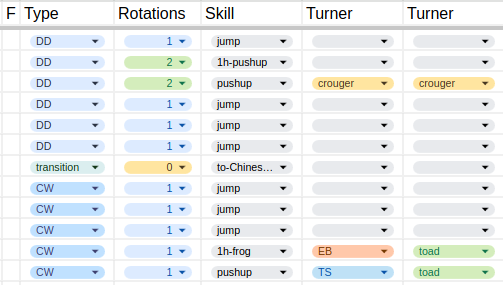
\includegraphics[width=0.7\linewidth]{img/doubledutch-matrix}
    \caption[skillmatrix-DD]{Representation of a skillmatrix used for Doube Dutch}
    \label{fig:doubledutch-skillmatrix}
\end{figure}

In addition, these skills can be combined with powers, releases\dots, and there are a number of special cases or exceptions that earn fewer or extra points. (Omitted in the MVP)
Put it all together, to create a skill matrix (work in progress), see double-dutch-matrix fig\ref{fig:doubledutch-skillmatrix}.

The skillmatrix for SR is still a little in progress since last year, knowing that some special cases can be omitted.

%\subsection{Skillafbakening \& branching}
%\label{subsec:video segmentation & branching}

% In \textcite{Zahan_2023} wordt het standaard LSTM uitgebreid om beter langdurige informatie te verwerken om resultaten van gehele gymnastiekoefening te voorspellen. Aangezien het jurysysteem van die data hierdoor één-op-één gekoppeld is aan het model, is dit niet robuust genoeg voor veranderende versies. Het proefconcept wenst dus de skills te leren waarop de levels gemapt worden via een functie.
    
% Om alle trucs en combinaties van elkaar te onderscheiden werd stap per stap een skillmatrix opgebouwd. Deze matrix tracht zo veel mogelijk, om niet te zeggen alle, oefeningen op te delen volgens kenmerkende eigenschappen. Dit denkproces bracht de afbakening van skills en combinaties in kaart.
% Freestyles en ander beeldmateriaal moet gesplitst worden in eenduidig, atomair benoembare (sub-)skills, minivideo's, die slechts één representatieve voorstelling hebben in de skillmatrix.
% Concreet betekent dit dat na afbakening van skills, iedere mini-video, nog herstelbaar moet zijn tot zijn combinatie.
% Doorgaans geeft het verlaten van de grond aan dat een truc begint, analoog bij het landen en in de lucht zijn. Dit is echter niet altijd het geval bij wraps of releases. Tevens moeten de geknipte video's, na de afbakening van de trucs, even lang zijn (gelijke dimensies). Een simpele truc hiervoor is het toevoegen van \emph{lege} informatie, zwarte frames, genaamd padden (Engelse term). Vaak zullen langdurige intervallen wraps of herstel van fouten zijn. Deze lange sequenties kunnen apart gemodelleerd worden of verder opgesplitst om de padding niet te lang te maken.

\subsubsection{Skillmatrix}

De de skillmatrix is voor verandering vatbaar, wanneer combinaties ontdekt worden die er niet in passen en ziet er op dit moment voor single rope als volgt uit:

\begin{itemize}
    \item \textbf{Description}: solely informative
    \item \textbf{Pointified notation}: Own notation for unique naming of skills
    \item \textbf{Category}: I, G, P, W, R, B, M, C, F
    \item \textbf{People}: skippers executing the skill (could be 2 or 3 in a team exercise)
    \item \textbf{mistakes}: skippers that made a mistake
    \item \textbf{Rotations}: rope rotations, 0-8
    \item \textbf{Rope direction first rotation}: forward, backward, side
    \item \textbf{Rope direction first rotation}: idem
    \item \textbf{Rope rotations switches}: 0 of 1, theoretical 2, 3, 4 possible
    \item \textbf{PBR}: 0,1,2+ parallel body-rotations with the ground (e.g. crab, push-up)
    \item \textbf{TTs}: 0.25 -> 2+ 'turntables' (e.g. hummingbird, 360, halve draai, turn table crab, turn table pushup)
    \item \textbf{multiplepart} 8x duplicated, one for each rope rotation, wrapstatus\dots
    \begin{itemize}
        \item \textbf{element} s, o, c, toad, EB, AS, TS, knee, straddle, mic, 1-H-release, powers, gyms \dots
        \item \textbf{switch} xAS, switch cross
        \item \textbf{wrapped bodyparts}: arm, leg, between leg around arm...
        \item \textbf{Interaction type}: scoop, take forward, take backward
    \end{itemize}
\end{itemize}

    
Skillmatrixes can change over time, initial skills not fitting the matrix will be left out for the MVP.
Furthermore, you see some labels can happen one at a time (cross-type), others (e.g. category) can happen at the same time (multi-branch output as described in section 4.4.1 \autocite{Coulibaly_2022}), others require softmax.

\subsection{Group activity}

As DD3 is a group activity, problems could arise while trying to detect skills. However, the hypothesis is that a DD3 freestyle always acts as one unit, thus not really requiring much special attention. This could pose a problem when adapting SR to SR2 where two individuals are not exactly one unit. Some further research can be done in models like stagNet \autocite{Qi_2020} can improve this.

\subsection{Challenges}
\label{subsec:challenges}

Unknown skills or special cases pose a problem. That's why the skillmatrix needs to defined in such a way that new combinations can fit the matrix as much as possible and/or in combination with zero-shot learning. (Sort of marking unique skills as 'I don't know' so that others new/unique ones will also be marked as 'I don't know')


\subsection{Summary literature}
\label{subsec:summary literature}

The PoC needs to localize the jumper, using existing models fine-tuned, segment actions, preferably through transfer-learning and using own splits or guessed splits to predict (sub)skills.
Predicted skills will then be mapped to their corresponding level.

% Refereren naar de literatuur kan met:
% \autocite{BIBTEXKEY} => (Auteur, jaartal): voor een referentie tussen
% haakjes, waar de auteursnaam GEEN onderdeel is van een zin.
% \textcite{BIBTEXKEY} => Auteur (jaartal): voor een narratieve referentie,
% waar de naam van de auteur effectief een onderdeel is van de zin.


%---------- Methodologie ------------------------------------------------------
\section{Methodology}%
\label{sec:methodoly}

After some more research about transformers and how to apply them for skill recognition and another non-transformer model besides convLSTM \& SAM to predict skills, the building process can started.
Using Canva, a \href{https://www.canva.com/design/DAGVz44QCgc/\_Mr9BrOqwwdy9cf-ieYFVg/edit?utm\_content=DAGVz44QCgc\&utm\_campaign=designshare\&utm\_medium=link2\&utm\_source=sharebutton}{user story map} is created to effectively see which tasks need to be done.

\subsection{General \& label location}

\begin{itemize}
    \item overview videos: navigate, filter, rename
    \item view video info, could have edit
    \item label inappropriate/blurry moments (idea: could be used, rather not)
    \item label passage/empty (livestream/wait) moments (idea: no skills)
    \item label jumper location
    \item Statistics of the general data distribution
\end{itemize}

\subsection{Predict location}

\begin{itemize}
    \item visualize jumpoer location predictions
    \item edit borders from new predictions
    \item visualize biggest localization mistakes (within video)
    \item visualize biggest localization mistakes (over all videos)
    \item localization model statistics
    \item data augmentation (if needed)
\end{itemize}

\subsection{Label action segments + label skills}

\begin{itemize}
    \item Label video action segment
    \item Loop-replay action segment
    \item Label segmented skills names
    \item mark false skills
    \item skills to level mapper (should have)
    \item search skills by name (could have)
    \item mark execution scale (could have)
    \item skilldistribution statistics (+/- distributionmatrix)
\end{itemize}

\subsection{Predict action segments}

\begin{itemize}
    \item visualize \& compare AI segmented skills
    \item visualize AI segmented skills from new videos (with confidence levels?)
\end{itemize}


\subsection{Predict skills}

\begin{itemize}
    \item model predicts levels (1-8 classes)
    \item model predicts variation element (4/6 classes)
    \item model predicts skill
    \item add judge scores to freestyles
    \item visualize \& compare AI labeled skills \& compare with total (judge)score
    \item validate AI recognized skills \& save as new training input
    \item label AI recognized skills as new or "i don't know"
    \item action segmentation stats
    \item skillrecognition stats
\end{itemize}


\subsection{Bis}

\begin{itemize}
    \item Language
    \item add competition jump order (easy recordings)
    \item stats competition
    \item insert multiple judge systems
\end{itemize}



\subsection{Answering sub-questions}
\label{subsec:methodology-sub-questions}

% TODO : finetune this : taal

To answer the questions; ``When are predictions good enough to serve as an additional juror or as a support tool?'' and ``Can we use the AI-Judge to improve jurors or vice versa?'', some suggestions can be made or a brainstorm with expert judges can be done. One suggestion is; that after submitting the score, the judge gets the levels of AI-Judge, which checks and indicates those levels that do not match their own given levels, judges can either improve themselves or improve the model. Subsequently, a transition can be made to verify the most uncertain skills of the model.

The sub-question on generalization to jury sports will have to wait and see how the pilot concept progresses.

\subsection{Training \& Hardware}

Working with videos alone requires a lot of resources, let alone training on the data with a normal laptop. It is best to work with one or more GPUs to aid the research process. In between, calculations can be made to estimate how long training sessions will take. This also gives a future reference for other computer vision concepts.


%---------- Verwachte resultaten ----------------------------------------------
\section{Expected results}
\label{sec:verwachte-resultaten}

Localization of the jumper shouldn't pose an issue. It's would be safe to say that a quick progression towards video action segmentation can be made. Even if segmented actions do not overlap with their actual skills, it's not that hard of a block for the skill recognition part. It would just mean, that skillrecognition can not be applied on new unsegmented videos.
It's expected that SAM will prove to give better results than his base convLSTM model and a transformer probably even better if correctly integrated.

On the long run, it's expected to surpass judges in accuracy.

To answer the questions asked in the introduction a list of unknown or potential answers.

\begin{itemize}
    \item How will the model be built? --> unknown
    \item What would be the main structure of the model? --> unknown
    \item Which human activity recognition examples can be used or altered as the base of the model? --> aligns with modelselection
    \item When are AI-recognitions acceptable to potentially use on competitions? --> when they score equally as good as a judge and can flag or anticipate unknowns.
    \item How much data is expected to increase the accuracy off the Judge. --> we'll know later
    \item How can we use the AI-Judge to improve judges? --> correcting/assisting them.
    \item What needs to changed to a working model, to apply it on other judge-sports such as gymnastics, synchronized swimming... --> define a skill-matrix \& data
\end{itemize}


\section{Expected conclusion}%
\label{sec:conclusion}

The AI-Judge can improve fairness of judging on competitions by annotating skills and, when expanded, giving confidence levels to the skills it predicted. Using AI-Judge, more transparency towards scores can increase competitiveness or enable the public to better understand the scores. Even using the model to display snapshots of freestyles along the predicted skill and confidence score in total.

This AI-Judge can be extended towards other disciplines or different sports like acro, figure skating, gymnastics or dressage, to achieve similar results.
    
The next steps will be extending freestyle judging into DD4, SR2 and special skills.
